\documentclass{article}
\usepackage[a4paper]{geometry}
\usepackage[brazil]{babel}
\usepackage[utf8]{inputenc}
\usepackage{url}
\usepackage{hyperref}
\usepackage{graphicx}
\usepackage{amsmath}
\usepackage{amsfonts}

\title{Atividade 2 - Programação Linear com Lazy Constraints}
\author{
	Felipe Pereira - RA: 263808 \\
	José Antonio Mauad Leis - RA: 219061 \\
	Lucas Guesser Targino da Silva - RA: 203534
}

\newcommand{\Set}[1]{\ensuremath{\left\{#1\right\}}}
\newcommand{\partsof}[1]{\ensuremath{\mathcal{P}\left(#1\right)}}
\newcommand{\Sum}[1]{\ensuremath{\displaystyle\sum\limits_{#1}}}
\newcommand{\abs}[1]{\ensuremath{\left| #1 \right|}}
\newcommand{\binary}{\ensuremath{\Set{0, 1}}}

\newcommand{\edge}{\ensuremath{e}}
\newcommand{\edges}{\ensuremath{E}}
\newcommand{\vertex}{\ensuremath{v}}
\newcommand{\vertices}{\ensuremath{V}}
\newcommand{\nvertices}{\ensuremath{\abs{\vertices}}}
\newcommand{\subvertices}{\ensuremath{S}}
\newcommand{\graph}{\ensuremath{G}}
\newcommand{\co}[1]{\ensuremath{c^{1}}}
\newcommand{\ct}{\ensuremath{c^{2}}}
\newcommand{\coe}{\ensuremath{c^{1}_{\edge}}}
\newcommand{\cte}{\ensuremath{c^{2}_{\edge}}}
\newcommand{\positiveReal}{\ensuremath{\mathbb{R}_+}}
\newcommand{\xoe}{\ensuremath{X^{1}_{\edge}}}
\newcommand{\xte}{\ensuremath{X^{2}_{\edge}}}
\newcommand{\de}{\ensuremath{D_{\edge}}}
\newcommand{\similarity}{\ensuremath{k}}
\newcommand{\totalconstraints}{\ensuremath{T_r}}
\newcommand{\bigo}[1]{\ensuremath{\mathcal{O}\left( #1 \right)}}

\begin{document}

\maketitle

\section{Enunciado do Problema}

Sejam:

\begin{enumerate}
    \item $\graph = \langle \vertices,\edges \rangle$: um grafo não-orientado completo:
    \begin{enumerate}
        \item $\vertices$: conjunto de vértices;
        \item $\edges$: conjunto das arestas;
    \end{enumerate}
    \item $\co , \ct: \edges \rightarrow \positiveReal$ duas funções custo nos vértices;
        \begin{enumerate}
            \item dada uma aresta $\edge$, escrevemos $c^{1}(\edge) = \coe$ e $\ct(\edge) = \cte$;
        \end{enumerate}
    \item $\similarity$: parâmetro de similaridade de ciclos;
\end{enumerate}

Objetivo: encontrar dois ciclos Hamiltonianos com custo total mínimo, tal que pelo menos $\similarity$ arestas do grafo sejam visitadas por ambos os ciclos.

\section{Modelo Matemático}

\subsection{Variáveis de Decisão}
\label{constraint:variables}

\begin{itemize}
	\item $\xoe$: presença da aresta $\edge$ no primeiro ciclo;
	\item $\xte$: presença da aresta $\edge$ no segundo ciclo;
	\item $\de$: presença de duplicação da aresta $\edge$;
\end{itemize}

Todas as variáveis de ``presença'' são decisões binárias com a seguinte interpretação de valores:

\begin{itemize}
	\item[0]: ausente
	\item[1]: presente
\end{itemize}

\subsection{Problema de Otimização}

Minimizar:
\begin{equation}
    \label{eq:goal}
 	\Sum{\edge \in \edges} \coe \ \xoe
 	+
 	\Sum{\edge \in \edges} \cte \ \xte
\end{equation}

Sujeito a:
\begin{equation}
	\label{constraint:vertex presence in 1}
	\Sum{\edge \in \delta(\vertex)} \xoe = 2
	\qquad
	\forall \vertex \in \vertices
\end{equation}

\begin{equation}
	\label{constraint:vertex presence in 2}
	\Sum{\edge \in \delta(\vertex)} \xoe = 2
	\qquad
	\forall \vertex \in \vertices
\end{equation}

\begin{equation}
	\label{constraint:no subcycle 1}
	\Sum{\edge \in \edges(\subvertices)} \xoe \leq \abs{\subvertices} - 1
	\qquad
	\forall
		\subvertices \subseteq \vertices,
		\subvertices \neq \vertices,
		\subvertices \neq \emptyset
\end{equation}

\begin{equation}
	\label{constraint:no subcycle 2}
	\Sum{\edge \in \edges(\subvertices)} \xte \leq \abs{\subvertices} - 1
	\qquad
	\forall
		\subvertices \subseteq \vertices,
		\subvertices \neq \vertices,
		\subvertices \neq \emptyset
\end{equation}

\begin{equation}
	\label{constraint:similarity compatibility}
	\xoe + \xte \leq 2 \ \de
	\qquad
	\forall \edge \in \edges
\end{equation}

\begin{equation}
	\label{constraint:similarity}
	\Sum{\edge \in \edges} \de \geq \similarity
\end{equation}

\begin{equation}
	\label{constraint:binary variables}
	\xoe, \xte, \de \in \binary
	\qquad
	\forall \edge \in \edges
\end{equation}

\subsection{Explicação das Restrições}

\begin{itemize}
    \item A função objetivo \eqref{eq:goal} é soma do custo de todas as arestas selecionadas.
    \item As restrições \eqref{constraint:vertex presence in 1} e \eqref{constraint:vertex presence in 2} garantem que a quantidade de arestas incidentes em todos os vértices seja 2, nos ciclos 1 e 2 respectivamente. Essa condição faz com que todos os vértices tenham que ser visitados (duas arestas pois uma é a de ``entrada'' e a outra a de ``saída'').
    \item As restrições \eqref{constraint:no subcycle 1} e \eqref{constraint:no subcycle 2} garantem que não existam subciclos nos ciclos. Nessas restrições, $\subvertices$ é um subconjunto próprio e não-vazio dos vértices do problema. A expressão $\edges(\subvertices)$ é o conjunto das arestas cujos vértices (ambos) estão em $\subvertices$.
    \item A restrição \eqref{constraint:similarity compatibility} garante que, se uma aresta foi escolhida para ser duplicada, então essa aresta aparecerá nos dois ciclos.
    \item A restrição \eqref{constraint:binary variables} garante que todas as variáveis são decisões binárias, ou seja, assumem apenas um de dois possíveis valores: 0 e 1.
\end{itemize}

\subsection{Tamanho das Restrições}

\begin{itemize}
	\item Restrições \eqref{constraint:vertex presence in 1} e \eqref{constraint:vertex presence in 2}: uma para cada vértice. Total: $2 \cdot \abs{\vertices}$;
	\item Restrições \eqref{constraint:no subcycle 1} e \eqref{constraint:no subcycle 2}: uma para $\subvertices \in \partsof{\vertices}, \subvertices \neq \vertices, \subvertices \neq \emptyset$. Total: $2 \cdot \left( 2^{\abs{\vertices}} - 2\right)$;
	\item Restrições \eqref{constraint:similarity compatibility}: uma para cada aresta. Total: $\abs{\edges} = \dfrac{\abs{\vertices}^2 - \abs{\vertices}}{2}$ (já que o grafo é completo);
	\item Restrições \ref{constraint:similarity}: apenas uma. Total: 1;
\end{itemize}

Assim, o número total de restrições é:

\begin{equation}
	\totalconstraints =
		  2 \cdot \abs{\vertices}
		+ 2 \cdot \left( 2^{\abs{\vertices}} - 2\right)
		+ \dfrac{\abs{\vertices}^2 - \abs{\vertices}}{2}
		+ 1
\end{equation}

Note que $\totalconstraints \in \bigo{2^{\nvertices}}$, isto é, há um número exponencial de restrições.

Na implementação computacional do problema, não é possível adicionar tantas restrições por falta de recursos computacionais (memória e processamento). Há entretanto uma forma de contornar o problema atŕavés do que se chama de \textit{lazy evaluation}. A ideia é não adicionar tais restrições no início. Conforme soluções factíveis são encontradas, verifica-se se há subciclos nelas e, caso sim, adiciona-se apenas as restrições necessárias para eliminar tais subciclos.

Dependendo do caso em mãos, essa abordagem pode reduzir drasticamente o número de restrições e consequentemente acelerar a busca.


\section{Experimento Computacional}

\subsection{Configuração da Máquina}

O problema foi executado num ideapad S145 81S90005BR: Lenovo IdeaPad S145 Notebook Intel Core i5-8265U (6MB Cache, 1.6GHz, 8 cores), 8GB DDR4-SDRAM, 460 GB SSD, Intel UHD Graphics 620.

O sistema operacional foi o Fedora 35 executando o Python 3.7.12 e Gurobi Optimizer v9.5.1rc2\cite{gurobi}.

Como linguagem de programação, utilizamos Python\cite{python3} pela facilidade de uso e disponibilidade de ferramentas.


\subsection{Dados do Problema}

Os dados do problema foram fornecidos em um arquivo contendo 4 colunas e 250 linhas. A interpretação dos dados é a seguinte: cada linha representa um vértice e cada par de coluna as coordenadas desse vértice. A razão para um vértice ter duas posições diferentes é simplesmente para que as distâncias entre eles tenham valores diferentes no primeiro e no segundo ciclo.

O modelo na verdade precisa apenas de pesos. Construímos a primeira função de custo como a distância euclidiana entre os pontos das colunas 1 e 2. Da mesma forma, utilizamos distância euclidiana entre os pontos das colunas 3 e 4 para construir a segunda função de custo.

Note que, com essa interpretação, parece que temos dois conjuntos de vértices, um definido pelas colunas 1 e 2, e outro definido pelas colunas 3 e 4. Conforme explicitado no primeiro parágrafo da seção, esse não é o caso. Cada linha é um vértice e os valores fornecidos servem apenas para calcular a distância euclidiana e usá-la como peso para as arestas. Dessa forma, a aresta que liga os vértices representados pelas linhas 12 e 84, por exemplo, possui dois pesos diferentes, um para ser utilizado no primeiro ciclo e outro para ser utilizado no segundo.

\subsection{Geração das Instâncias}

Para gerar instâncias de um dado tamanho $N$, utilizamos as primeiras $N$ linhas dos dados fornecidos.

\section{Resultados}

\subsection{Resultados Obtidos}

O programa foi construído para processar todas as instâncias e parâmetros pedidos no exercício. Mas devido a restrições computacionais, não conseguimos executar os dois últimos (Vertíces-250 \& Similaridade-0.5, Vértices-250 \& Similaridade-1). Abaixo podemos ver a Tabela~\ref{f:dados}  dos resultados obtidos.
\begin{figure}
    \centering
    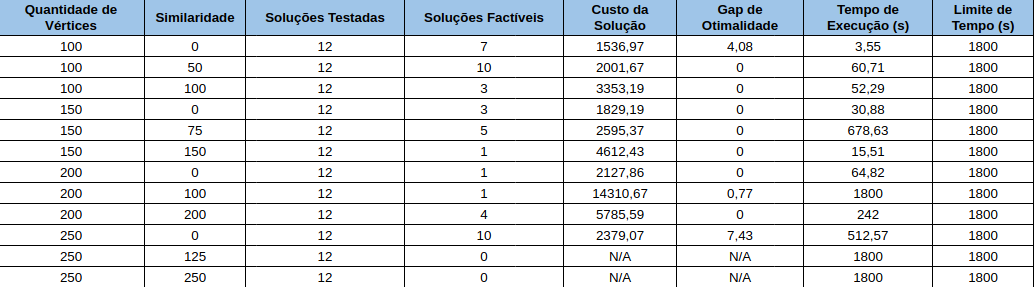
\includegraphics[width=0.7\textwidth]{figures/resultados.png}
    \caption{Resultados da Execução}
    \label{f:dados}
\end{figure}

Podemos notar que, mesmo com o $k$ similar, o aumento no número de Vértices também gera aumento do custo da solução, o que já era esperado pela teoria, conforme demonstrado na Tabela~\ref{f:tab-execucao}:

\begin{table}[]
\label{t:custo}
\centering
\begin{tabular}{c|c|c}
            & \multicolumn{2}{c}{Custo Mínimo} \\ \hline
\# Vértices & K  & Custo \\ \hline
100         & 0       & 1536,97 \\ \hline
150         & 0       & 1829,19 \\ \hline
200         & 0       & 2127,86 \\ \hline
250         & 0       & 2379,07 \\ \hline
100         & 0.5     & 2001,67 \\ \hline
150         & 0.5     & 2595,37 \\ \hline
200         & 0.5     & 14310,67\\ \hline
250         & 0.5     & N/A     \\ \hline
100         & 1       & 3353,19 \\ \hline
150         & 1       & 4612,43 \\ \hline
200         & 1       & 5785,59 \\ \hline
250         & 1       &   N/A
\end{tabular}
\caption{Custo da soluções por Vértice/Similaridade}
\label{f:tab-execucao}
\end{table}

Com isso, foi possível compilar o custo da solução, de acordo com os parâmetros de Vértices e Similaridade, conforme a Figura~\ref{f:g-custo}
\begin{figure}
    \centering
    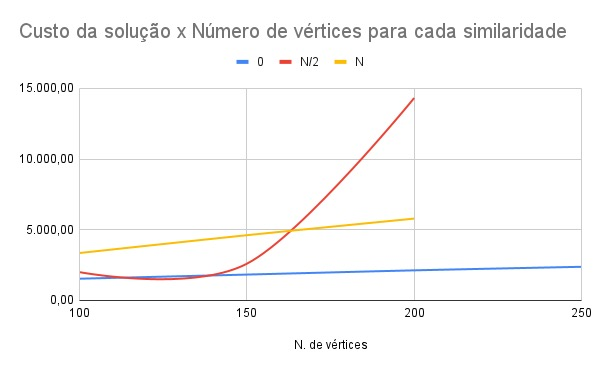
\includegraphics[width=0.7\textwidth]{figures/sol-custo.jpeg}
    \caption{Resultados da Execução}
    \label{f:g-custo}
\end{figure}

Assim como a relação do aumento de complexidade com o Tempo de Execução, conforme a Figura~\ref{f:g-tempo}
\begin{figure}
    \centering
    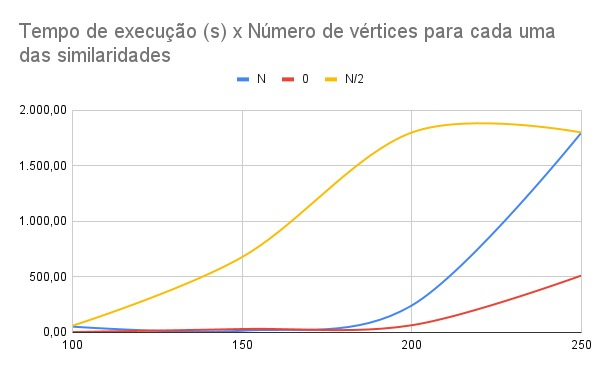
\includegraphics[width=0.7\textwidth]{figures/sol-tempo.jpeg}
    \caption{Resultados da Execução}
    \label{f:g-tempo}
\end{figure}

\section{Análise e Observações Finais}

Podemos notar, ao avaliar o resultado das observações, que, para cada conjunto de vértices (em nosso caso: 100, 150, 200 e 250) temos um custo crescente com a adição de complexidade, ou seja, tanto com a adição de vértices, quanto com o aumento da similaridade (onde $k$ pode ser igual a {0, 0.5, 1}).

O aumento do custo da solução parece guardar uma relação linear com o aumento de vértices, embora fosse possível especular que a relação fosse exponencial a priori, dado o aumento da complexidade da solução. O mesmo é válido para o aumento da similaridade, representada pela variável $k$. O aumento do parâmetro de similaridade parece guardar uma relação linear de aumento com o custo da solução obtida.

O mesmo não pode ser dito em relação ao tempo computacional gasto para calcular as soluções. O tempo cresce exponencialmente de acordo com o aumento da complexidade da soluções, que é dada pela quantidade de vértices e pela similaridade entre os dois ciclos.

Este tipo de comportamento fez com que não conseguíssemos calcular as soluções para $k$=0.5 e $k$=1 para $V$=250. É importante notar que o enunciado do exercício nos colocou uma restrição de tempo de execução da busca por soluções em 30 minutos, ou seja, dentro deste tempo, o algoritmo não foi capaz de encontrar soluções viáveis para o problema. Testes com tempos maiores são recomendados para que se encontrem os resultados destas combinações.


\bibliographystyle{ieeetr}
\bibliography{bibliography}

\end{document}
